\section{Program Slicing}
\label{sec:slicing}    

    % Program Slicing

    Le \emph{program slicing} \cite{Wei81} est le calcul du sous-ensemble d'un
    programme qui affecte les valeurs de variables données à un point donné
    dans son exécution. Le sous-ensemble du programme, appelé {\em slice}, est
    lui-même un programme dont l'exécution produit les mêmes valeurs que le
    programme original pour les variables données au point donné. 
    Un \emph{slice} est calculé vis-à-vis d'un critère de \emph{slice}
    $\mathcal{C} = \langle l, v \rangle$ avec $l \in \mathcal{L}$ une étiquette
    et $v \subseteq \mathcal{V}$ un ensemble de variables. Ainsi, si on
    considère le programme de la figure~\ref{fig:dump} et le critère de $slicing$, $\langle 3030,
    \{ctr \}\rangle$, c'est à dire la valeur du registre $ctr$ %\footnote{Sur PowerPC,
%    le $ctr$, pour CounT Register est décrémenté et testé par l'instruction de
%    branchement conditionnel $bdnz$}. 
    lorsque le pointeur d'instruction contient
    l'adresse $3030$, on obtient le slice présenté figure~\ref{fig:slice2}. En effet, l'instruction $bdnz$ modifie $ctr$, $ctr$ a été affecté en $3018$ à partir de $r8$ et $r8$ a été affecté en $3010$.
    
    Il existe différentes approches permettant de calculer un \emph{slice}
    \cite{Tip95}.  Cependant, seule la sous catégorie des approches basées sur
    la manipulation de graphes permet de calculer un \emph{slice} pour les
    fichiers binaires exécutables. Nous nous basons plus précisément sur une
    approche permettant de calculer des \emph{slices} précis pour les
    programmes composés de plusieurs procédures (\emph{program slicing}
    interprocédural) \cite{KJL03}.

    %Les figures
    %\ref{fig:slice1} et \ref{fig:slice2} donnent les \emph{slices} du programme
    %\texttt{fibcall-O2.elf} (cf. figure \ref{fig:dump}) respectivement pour le
    %critère $\mathcal{C} = \langle 302c, \{ r10 \} \rangle$ et le critère
    %$\mathcal{C} = \langle 3030, \{ ctr \} \rangle$. $R$ est l'ensemble des
    %variables -- ou registres ici -- explicitement ou implicitement manipulés
    %qui font l'objet de dépendances de données entre les différents blocs de
    %base du CFG. Autrement dit, ce sont les variables qui sont à conserver dans
    %l'espace d'état du système pour en réaliser une analyse précise et efficace
    %vis-à-vis de leurs valuations possibles.

          %$R = \{\}$}
        %$R = \{ctr\}$}
    \begin{figure}[ht]
      \centering
      \begin{subfigure}[t]{.20\textwidth}
        \centering
        \captionsetup{justification=centering}
        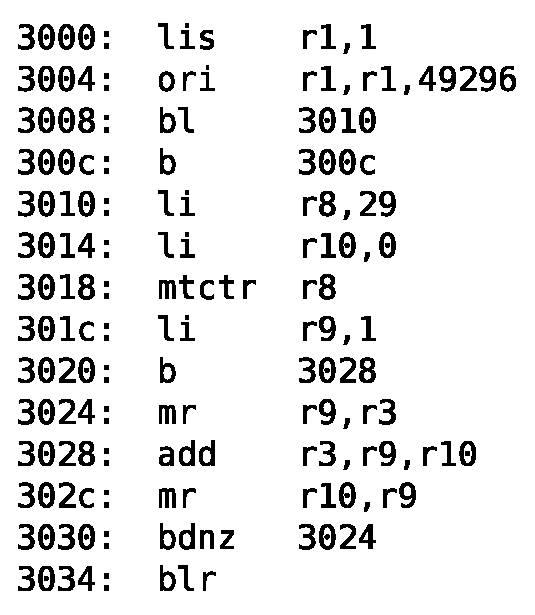
\includegraphics[scale=.4]{img/dump.eps}
        \caption{\emph{dump} de \texttt{fibcall-O2.elf}} %\\
         % $R = \{r3, r8, r9, r10, ctr\}$}
        \label{fig:dump}
      \end{subfigure}
      \begin{subfigure}[t]{.20\textwidth}
        \centering
        \captionsetup{justification=centering}
        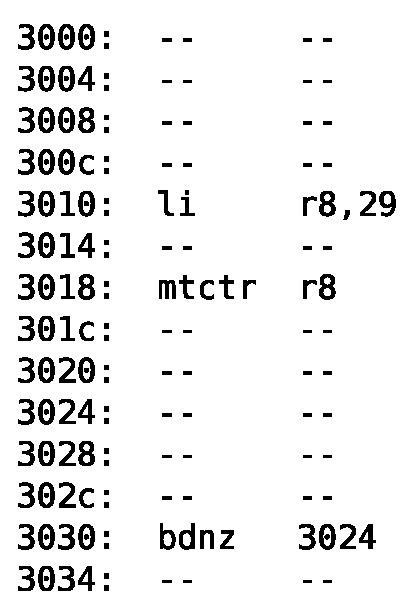
\includegraphics[scale=.4]{img/slice2.eps}
        \caption{$\mathcal{C} = \langle 3030, \{ ctr \} \rangle$}% \\
        \label{fig:slice2}
      \end{subfigure}
      \caption{Exemple de \emph{slice} portant sur la condition de branchement}
    \end{figure}

    %% Quand le \emph{slicing} s'applique à une seule procédure monolithique on
    %% parle de \emph{slicing} intraprocédural. En revanche lorsque le
    %% \emph{slicing} s'applique à un programme entier, au delà des frontières
    %% d'une procédure, on parle de \emph{slicing} interprocedural.
  
    % Intérêt du Program Slicing des CFG pour la vérification de modèle.

    Dans notre cas, nous utilisons le \emph{program slicing} pour identifier
    les variables du programme qui influent sur son flot de contrôle. En effet,
    seules ces variables sont à inclure dans l'espace d'état du modèle du code
    binaire qui sera fourni à la chaîne de calcul de borne sur le pire temps
    d'exécution. Toutes les autres variables peuvent être abstraites,
    c'est-à-dire qu'il ne sera pas nécessaire de retenir leur valeur après
    avoir \og exécuté \fg une instruction les définissant. Le modèle du code
    binaire étant ensuite destiné à être composé avec les modèles du matériel,
    cette réduction de la taille de son espace d'état a un impact très
    significatif sur la réduction de la taille de l'espace d'état du modèle à
    analyser.

    Pour déterminer l'ensemble des variables à conserver, il faut calculer une
    slice pour toutes les étiquettes correspondants à des instructions de
    branchement conditionnels, en choisissant comme variable les registres sur
    lesquels est évalué la condition. Si l'on considère le programme de la
    figure~\ref{fig:dump}, il comporte un seul branchement conditionnel :
    l'instruction \verb|bdnz 3024| à l'adresse $3030$. Ce branchement est pris
    si le registre de comptage \verb|ctr| est non nul. Pour calculer les
    variables à garder, il faut donc calculer la slice correspondant au critère
    $\langle 3030, \{ctr\} \rangle$. Elle est donnée figure~\ref{fig:slice2}.
    L'ensemble des variables manipulées (explicitement ou implicitement) dans
    le programme initial est $\{r1, r3, r8, r9, r10, lr, ctr\}$. Le
    sous-ensemble à conserver dans le modèle est $\{r8, ctr \}$.

    %Pour pallier au problème de l'explosion de l'espace d'état inhérent à la
    %vérification des modèles il est nécessaire de réduire au maximum la quantité
    %d'informations définisant l'état du système. Une utilisation spécifique du
    %\emph{program slicing} permet de ne conserver dans l'espace d'état
    %du système uniquement les informations définissant l'état des variables --
    %registre ou contenu de la pile -- dont la valuation influt directement sur
    %le flot de contrôle.

    %Il n'est, en effet, pas nécessaire de conserver dans l'espace d'état du
    %système les valuations de toutes les variables qui n'agissent pas
    %directement sur le flot de contrôle puisqu'elles n'influent pas sur le temps
    %d'exécution. Le \emph{slice} donné en figure \ref{fig:slice2} contient
    %l'ensemble des instructions du programme \texttt{fibcall-O2.elf} qui agissent
    %directement sur le flot de contrôle et manipulent des variables explicitement
    %ou implicitement. Il est donc nécessaire de conserver dans l'espace d'état
    %du système uniquement la valuation d'un seul registre ($R = \{ ctr$ \}) au
    %lieu des 7 registres originaux ($R = \{r1, r3, r8, r9, r10, lr, ctr\}$,
    %cf. figure \ref{fig:dump}).
     
    %\vspace{1em}
  
    % Program Slicing à base de graphes

    
    %% L'algorithme de \emph{slicing} implémenté s'appuie sur la méthode évoquée
    %% ci-après -- cf. \cite{CF97}. Les dépendances de données du programme y sont
    %% représentées par l'arbre post-dominateur et par des chaines de
    %% \emph{use-definition}. Ces chaines relient chaque utilisation d'une
    %% variable aux définitions qui peuvent l'affecter.

    %% Les dépendances de contrôle du programme sont manipulés à travers un graphe
    %% de dépendance de contrôle. Un graphe de dépendance de contrôle est un graphe
    %% où les arcs signifient un lien de dépendance entre la valuation du n{\oe}ud
    %% origine et l'exécution du n{\oe}ud cible.
    
